\setcounter{ExampleCounter}{1}
Let us start with the basics. What is statistics? The field of \textbf{statistics} encompasses collecting, organizing, analyzing and presenting data. \textbf{Data} is simply
collected information. That information can be collected via surveys, polls, records, experiments, studies, or censuses, just to name a few. A \textbf{census} is when we collect data on the entire population, polling each and every individual. As you can imagine, that would take a lot of time and resources. \marginnote{The 2010 census cost about \$13 billion to administer}That is why in the United States, a census occurs only every 10 years. In all other situations, we do what is known as sampling, where we assume that if we study a small portion of the total group, the results will be similar to what we would find if we polled the entire group.

Our goal in statistics, then, is to select a good sample, gather data from the sample, organize and summarize the data, and draw conclusions from the sample about the total population.

\subsection{Population and Sample}

A \textbf{population} is a collection of persons or objects under study. To study the population, we select a \textbf{sample}. The idea of \textbf{sampling} is to select a portion (or subset) of the larger population and study that portion (the sample) to gain information about the population. Sampling is a very practical technique. If you wished to find the average height of students at your school, you probably wouldn't collect data from every single student; this wouldn't be very feasible. It would make more sense to select a sample of students. The data collected would be the students' heights.  In presidential elections, opinion polls sample 1000 to 2000 people. The opinion poll is supposed to represent the views of the people in the entire country. Manufacturers of ice cream take samples to determine if a pint of ice cream actually contains a pint of ice cream.

\begin{example}[https://www.youtube.com/watch?v=-AK3lL3YKOA]{Pet Ownership}
A sample of 2,000 households in the U.S. was selected and asked if they currently own at least one pet. The results show that 69\% of households do own at least one pet.
Identify the sample and population in this situation.\\


\marginnote{\bfseries Solution}
The sample is the 2,000 households and the population is all households in the U.S. Notice that even though the population is not explicitly stated, we can infer it from carefully reading the sentence. 
\end{example}

\begin{try}[http://www.izzomath.com/103text/stats/example1.1/story.html]
A researcher wants to know how citizens of Frederick City felt about a voter initiative. To study this, she goes to the Francis Scott Key Mall in the city, randomly selects 500 shoppers and asks them their opinion. Sixty percent indicate they are supportive of the initiative. What is the sample and population?:
\end{try}

Let's go back and think about finding the average height of students at your school. How would you go about obtaining your sample? Would you sample all your friends, or all your classmates? How about asking people in the library on a Wednesday afternoon? Would any of these sampling techniques give you a good estimate of the average height of all students? 


We have to make sure our sample is not \textbf{biased}, or leaning in a certain direction. Maybe you like to hang out with tall people and all your friends are tall. Maybe only 10 people are in the library on Wednesdays. Your sample must be random and representative in order to get a good estimate of the population data.  A sample is \textbf{random} if everybody in the population has the same chance of being selected into the sample. A sample is \textbf{representative} if it contains the characteristics of the population.

\begin{proc}{Random Samples}
The key to a random sample is that each member of the population is equally likely to be selected.

\paragraph{Examples of Random Samples}
\begin{itemize}
\item If the population is students in a particular classroom, number the students in the classroom from 1 to $n$ and use a random number generator to select numbers between 1 and $n$.
\item If the population is FCC students, list their FCC email accounts and number them, then pick random numbers between 1 and $n$, where $n$ is the number of students.
\end{itemize}

\paragraph{Examples of Biased Samples}
\begin{itemize}
\item \marginnote{Not every resident of the county has a phone, let alone a phone listed in the phone book}If the population is residents of Frederick County, number the entries in the phone book and use a random number generator to select a sample.
\item If the population is American citizens, go to the entrance of Yankee Stadium and poll everyone entering.
\item If the population is FCC students, poll the students in one class.
\end{itemize}

If you're ever unclear on whether or not a sampling method is random, simply ask whether or not every member of the population has an equal chance of being selected.  A random sample gives better results than a biased sample because characteristics that could muddy the results of the study get averaged out by the randomness.
\end{proc}
\vspace{0.5in}

\subsubsection*{Picking Random Numbers with a TI-83}
Your graphing calculator can select random numbers.  To access this menu, press the MATH button and use the left and right arrows to navigate to the PRB tab (PRB for probability).
\begin{center}
\begin{tabular}{l b{0.6\textwidth}}
\includegraphics[width=0.3\textwidth]{RandMenu} & Selecting \texttt{rand} will select a ``random'' (technically pseudo-random, but close enough for us) number between 0 and 1.  Selecting \texttt{randInt(} will allow you to choose a random integer between a given lower and upper bound, or several of those.
\end{tabular}
\end{center}

\begin{center}
\begin{tabular}{l b{0.6\textwidth}}
\includegraphics[width=0.3\textwidth]{RandInt} & To select a single random integer, enter \texttt{randInt(}lower bound\texttt{,}upper bound\texttt{)}, with whatever numbers you want for the lower and upper bounds.  To select $n$ random integers, enter \texttt{randInt(}lower bound\texttt{,}upper bound\texttt{,}$n$\texttt{)}
\end{tabular}
\end{center}
\vfill
\pagebreak

\begin{example}[https://www.youtube.com/watch?v=mm1iQfMgNHE]{Cartwheels}
A coach is interested in how many cartwheels the average college freshman can do at his university. Eight volunteers from the freshman class step forward. After observing their
performance, the coach concludes that college freshmen can do an average of 16 cartwheels in a row without stopping. Is this sample random and representative?\\

\marginnote{\bfseries Solution}
The population is the class of all freshmen at the coach's university. The sample is composed of all freshmen so that is good. However, the sample is poorly chosen because volunteers are more likely to be able to do cartwheels than the average freshman: people who cannot do cartwheels probably did not volunteer! Hence, this sample is not random. We are also not told of the gender of the volunteers. Were they all women, for example? That might affect the outcome (if the school is co-ed). We cannot be sure this sample is representative.

\end{example}

\begin{try}[http://www.izzomath.com/103text/stats/example1.2/story.html]
A substitute teacher wants to know how students in the class did on their last test. The teacher asks the 10 students sitting in the front row to state their latest test score. He concludes from their responses that the class did extremely well. What is the sample and population? Is the sample random and representative? Why or why not?
\end{try}

In general, self-selected samples (or volunteer samples) are not representative of the population.  For this reason, surveys with voluntary responses are not reliable.  People who volunteer their opinion for online reviews, for instance, tend to be strongly positive or negative; the voluntary sample misses everyone in the middle who doesn't have a strong opinion.

The most famous example of this comes from the 1936 presidential election, where the incumbent Democrat, Franklin D. Roosevelt, was challenged by the Republican governor of Kansas, Alf Landon.  The \textit{Literary Digest}, a weekly magazine, boasted that it had correctly predicted the results of the last 4 elections by sending out questionnaires to its huge sample of readers.  In 1936, the \textit{Digest} sent out 10 million questionnaires and received over 2 million responses, predicting that Landon would unseat Roosevelt with a handy victory.  When Election Day came, though, Roosevelt received over 60\% of the popular vote, carrying every state except for Maine and Vermont (including Landon's home state).  It was one of the most lopsided victories in U.S. history.  The reason for the failure of this poll was largely based on the voluntary response nature--those who responded were more likely to be those who were unhappy with the current administration; people who were happy with Roosevelt's programs had no incentive to fill out the questionnaire and send it in.

Largely due to this failure and embarrassment, the \textit{Literary Digest} folded within a few years.  In contrast, a young pollster named George Gallup (whose name is borne by the Gallup polls today) made his name in the 1936 election by correctly predicting the winner with a much smaller, carefully chosen sample.

\subsection{Frequency Distributions}

One of the most fundamental parts of statistics is presenting data clearly. After the data has been collected, it must be presented in a way so that it conveys all the necessary information and is easy for the viewer to understand. It is usually impractical and unhelpful to list all of the data that we gather for our audience; imagine gathering data on standardized test scores in a state and listing thousands of unsorted scores--there would be no way to make sense of the data.  When we present data, we want to show a clear picture of what's going on, without overwhelming our audience with so much data that the reality gets lost in the noise.


The first way that we'll present data is with a \textbf{frequency distribution}, which simply counts how often each data value occurs.  For instance, suppose twenty students were asked how many hours they worked per day. Their responses, in hours, are as follows: \[5, 6, 3, 3, 2, 4, 7, 5, 2, 3, 5, 6, 5, 4, 4, 3, 5, 2, 5, 3.\]
\pagebreak

The table below lists the different data values in ascending order and their frequencies.

\begin{center}
\begin{tabular}{c | c}
\textbf{Data Value} & \textbf{Frequency}\\
\hline
2 & 3\\
3 & 5\\
4 & 3\\
5 & 6\\
6 & 2\\
7 & 1
\end{tabular}
\end{center}

If one data value between 2 and 7 didn't appear in the data set--for example, if none of the students responded that they worked 4 hours per day--we would usually still include the row for 4 and just note that the frequency was 0 for that value.

The \textbf{frequency} is the number of times a data value occurs. According to the table above, there are three students who work two hours, five 
students who work three hours, and so on. The sum of the values in the frequency column, 20, represents the total number of students included in
the sample. 

We can also calculate the \textbf{relative frequency} of each value, which is the ratio of the number of times a value occurs to the total number of outcomes. We can include these in a third column on our frequency table.  To find the relative frequencies, divide each frequency by the total number of students in the sample--in this case, 20. Relative frequencies can be written as fractions, decimals, or as in the table below, as percents.
\begin{center}
\begin{tabular}{c | c | c}
\textbf{Data Value} & \textbf{Frequency} & \textbf{Relative Frequency}\\
\hline
2 & 3 & 3/20 or 15\% \\
3 & 5 & 5/20 or 25\% \\
4 & 3 & 3/20 or 15\% \\
5 & 6 & 6/20 or 30\% \\
6 & 2 & 2/20 or 10\% \\
7 & 1 & 1/20 or 5\%
\end{tabular}
\end{center}
The sum of all the values of the relative frequency column of the table above is 20/20, or 1.  Note, because of rounding, the relative frequency column may not 
always sum to one. However, it should be close to one.


\begin{example}[https://www.youtube.com/watch?v=VQhKtct3nog]{Daily Commute}
Nineteen people were asked how many miles, to the nearest mile, they commute to work each day. They responded as follows: \[2, 5, 7, 3, 2, 10, 18, 15, 20, 7, 10, 18, 5, 12, 13, 12, 4, 5, 10.\] This is summarized in the frequency table below:

\begin{center}
\begin{tabular}{c | c | c}
\textbf{Data Value} & \textbf{Frequency} & \textbf{Relative Frequency}\\
\hline
3 & 3 & 3/19 \\
4 & 1 & 1/19 \\
5 & 3 & 3/19 \\
7 & 2 & 2/19 \\
10 & 3 & 4/19 \\
12 & 2 & 2/19 \\
13 & 1 & 1/19 \\
15 & 1 & 1/19 \\
18 & 1 & 1/19 \\
20 & 1 & 1/19  
\end{tabular}
\end{center}

\begin{itemize}
\item Is the table correct? If it is not correct, what is wrong?\\

It is incorrect, because the frequency column sums to 18, not 19 as it should.  One of the data values was left out.  Besides, two people responded that they commute 2 miles, and that doesn't appear on the table at all.\\

\item True or false: Three of the people surveyed commute three miles. If the statement is not correct, what should it be? If the table is incorrect, make the corrections.\\

False.  The frequency for 3 miles should be 1.  When building the table, the two that responded 2 miles got lumped into the 3 category.\\

\item What fraction of the people surveyed commute five or seven miles?\\

5/19\\

\item What fraction of the people surveyed commute 12 miles or more? Less than 12 miles? Between 5 and 13 miles (not including those who commute exactly 5 or exactly 13 miles)?\\

7/19, 12/19, 7/19
\end{itemize}
\end{example}

Sometimes, it's more practical to make a \textbf{grouped frequency distribution}, where the frequencies are not single numbers, but groups of numbers.

For instance, suppose you gathered data on how long it took you to get ready in the morning.  For 40 days, you measured the amount of time between when your alarm went off and you left the house, and you got the following results in minutes:
\begin{center}
\begin{tabular}{c c c c c c c c c c}
35.6 & 28.7 & 25.5 & 23.2 & 23.7 & 32.1 & 29.6 & 19.5 & 21.4 & 13.6\\
24.9 & 26.7 & 25.8 & 31.8 & 30.4 & 20.1 & 25.3 & 29.9 & 37.5 & 26.6\\
32.3 & 36.5 & 18.5 & 17.7 & 15.2 & 24.7 & 21.4 & 16.6 & 19.5 & 30.3\\
38.7 & 27.4 & 22.9 & 24.6 & 28.5 & 17.5 & 31.4 & 32.2 & 21.6 & 28.4\\
\end{tabular}
\end{center}

If we built a frequency distribution with one row for each distinct value, the table would not give any useful information; it wouldn't serve the purpose of a frequency distribution, which is to give a preliminary idea of where the data is clustered and where it is spread out.

Instead, we can make a grouped frequency distribution by grouping together data values in the same range.  If we do this for the data set above by grouping in sets of 5, we get the grouped frequency distribution below.
\begin{center}
\begin{tabular}{c | c}
\textbf{Data Values} & \textbf{Frequency}\\
\hline
10--less than 15 & 1\\
15--less than 20 & 7\\
20--less than 25 & 10\\
25--less than 30 & 11\\
30--less than 35 & 7\\
35--less than 40 & 4\\
\end{tabular}
\end{center}

This distribution has six categories, called \textbf{classes}.  The starting values of the classes (10, 15, 20, etc.) are called the \textbf{lower class limits}, and the ending values are called the \textbf{upper class limits}.  The \textbf{class width} is the difference between the lower class limits.  Notice that if we subtract $20-15$, we get 5.  Therefore, the class width in this example is 5.

\begin{proc}{Choosing Classes}
When building a grouped frequency distribution, you'll usually have the freedom to choose how you want to separate the classes.  Here are some guidelines you should follow:
\begin{itemize}
\item Each class should be the same width.  Notice in the example above that each class was five units wide.  If not, the grouped frequency distribution would not give a clear picture of how the data is arranged.
\item Classes cannot overlap.  In the example above, we avoided overlap by letting the first class go up to ``less than 15'' and having the second class start at 15, and similarly for the other classes.  If the classes overlapped at 15, it wouldn't be clear into which category we should place a data value of 15.0.
\item Avoid empty classes if possible.  This can occur if you choose to have too many classes.
\item Don't make open-ended classes.  For instance, in the example above we didn't make the last class ``35 and above,'' which would have been an open-ended class.  The reason not to do this is that it violates the first guideline about having all classes have the same width.
\end{itemize}
\end{proc}

To find the appropriate class width to use, you can start by deciding on the number of classes you want to use. In our example above, we chose 6. Then the class width is found by dividing the distance from the minimum to the maximum by the number of classes. 

\begin{formula}{Class Width}

\[\textrm{Class Width } = \dfrac{\textrm{Maximum - Minimum}}{\textrm{Number of Classes}}\]
Round UP to the next whole number.
\end{formula}

\subsection{Histograms}

Let's revisit the example we looked at earlier of the twenty students and the number of hours worked each day.
\begin{center}
\begin{tabular}{c | c}
\textbf{Data Value} & \textbf{Frequency}\\
\hline
2 & 3\\
3 & 5\\
4 & 3\\
5 & 6\\
6 & 2\\
7 & 1
\end{tabular}
\end{center}

We can represent a frequency distribution with a picture instead of a list of numbers, which is helpful to our visual-oriented brains.  The graph we build from a frequency distribution is called a \textbf{histogram}.  A histogram is a bar graph\marginnote{Note carefully: a \textbf{bar graph} has gaps between the bars.  A \textbf{histogram} (what we do in this chapter) has no gaps.} with a bar for each class in the frequency distribution, and the height of the bar represents the frequency listed for that class.

The vertical axis is labeled either frequency or relative frequency, the horizontal axis is labeled with what the data represents (for instance, hours worked per day). The histogram from the working hours frequency distribution is below: 

\begin{center}
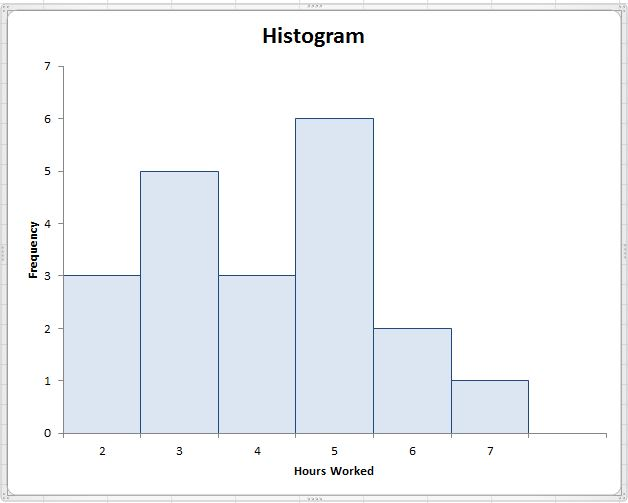
\includegraphics[scale=0.6]{HoursWorkedHistogram}
\end{center}

\begin{proc}{Using Your Calculator}
The TI calculator will construct a histogram for you.  You have two options: entering the frequency distribution into the calculator, or entering the raw data and letting the calculator find the frequency of each value.

\paragraph{Option 1:} Enter the frequency distribution
\begin{enumerate}
\item Press the \textbf{STAT} button to enter the statistics menu
\item Choose the \textbf{Edit} option to edit the data list
\item Enter the classes (or values if it isn't a grouped table) into L1 and enter the frequency into L2
\item Choose the \textbf{STATPLOT} option by clicking the \textbf{2nd} and \textbf{Y=} buttons
\item Turn Plot1 On and choose the histogram option, with the data (Xlist) in L1 and the frequency in L2
\item Press \textbf{ZOOM} and choose the "ZoomStat" option
\end{enumerate}
By pressing the \textbf{TRACE} button, you can see the frequency of the bars.\\

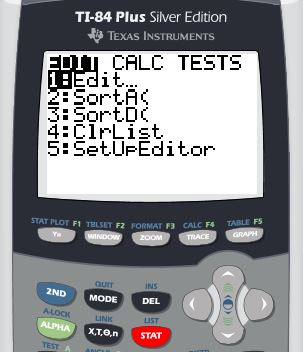
\includegraphics[height=1.25in]{Calc1}
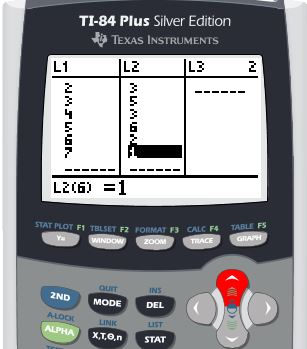
\includegraphics[height=1.25in]{Calc2}
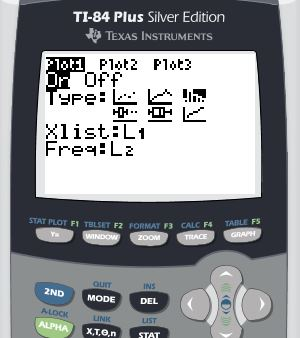
\includegraphics[height=1.25in]{Calc3}
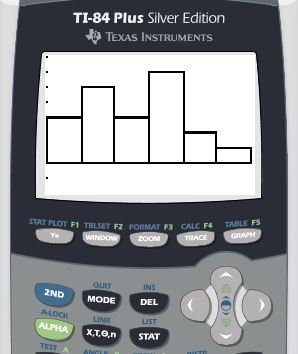
\includegraphics[height=1.25in]{Calc4}

\paragraph{Option 2:} Enter the raw data\\

Instead of using L1 and L2, simply enter the data into L1 and enter ``1'' for the Freq option when creating the histogram.  You can change the width of the classes by changing Xscl under the \textbf{WINDOW} menu.
\begin{center}
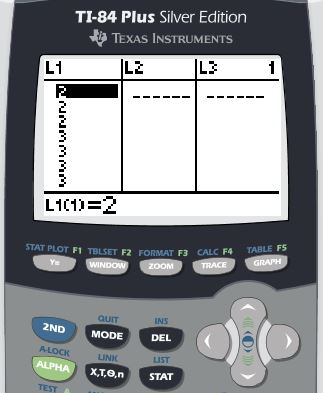
\includegraphics[height=1in]{Calc2b}
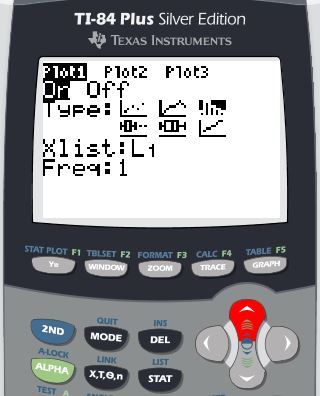
\includegraphics[height=1in]{Calc3b}
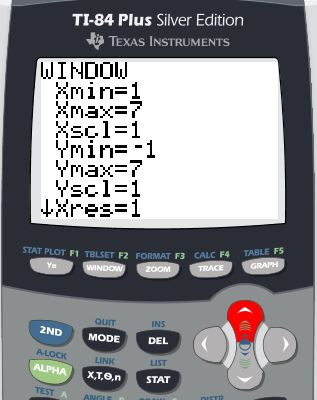
\includegraphics[height=1in]{Calc4b}
\end{center}
\end{proc}
\vspace{0.5in}

The graph below was created by the TI-83 using the data about getting ready in the morning, by entering the raw data in L1:
\begin{center}
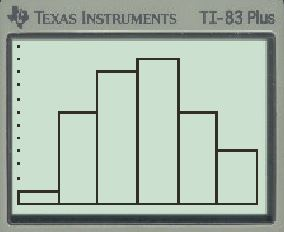
\includegraphics[scale=1]{Calc5}
\end{center}
\vfill
\pagebreak

\subsection{Stem-and-Leaf Plots}
There is one major downside to grouped frequency distributions: some of the data gets lost in the summary.  In other words, maybe in an example all we know is that there are 10 observations between 20 and 25, but we don't know exactly what all those observations are.  This is an example of the trade-off between clarity and precision: often, the more precise we are, the less clear our summary will be.

To split the difference and display the data in a way that exhibits where it is clustered without losing any information about the data is to use a \textbf{stem-and-leaf} plot.  Here, the data is grouped by tens; each tens value is a stem, and all the data points that have that tens value are listed as the leaves.  We'll illustrate with an example, using the same data set we used to construct the grouped frequency distribution above, but this time without the decimal places:
\begin{center}
\begin{tabular}{c c c c c c c c c c}
35 & 28 & 25 & 23 & 23 & 32 & 29 & 19 & 21 & 13\\
24 & 26 & 25 & 31 & 30 & 20 & 25 & 29 & 37 & 26\\
32 & 36 & 18 & 17 & 15 & 24 & 21 & 16 & 19 & 30\\
38 & 27 & 22 & 24 & 28 & 17 & 31 & 32 & 21 & 28\\
\end{tabular}
\end{center}

The tens places are 1, 2, and 3, and each of them gets a category:
\begin{center}
\begin{tabular}{r | l}
Stems & Leaves\\
\hline
1 & {\color{white}3 5 6 7 7 8 9 9}\\
2 & {\color{white}0 1 1 1 2 3 3 4 4 4 5 5 5 6 6 7 8 8 8 9 9}\\
3 & {\color{white}0 0 1 1 2 2 2 5 6 7 8}
\end{tabular}
\end{center}

Finally we go through (carefully) and find each value that begins with a 1 and list the ones place of each of them under the first category, and similarly with the other two categories.
\begin{center}
\begin{tabular}{r | l}
Stems & Leaves\\
\hline
1 & 3 5 6 7 7 8 9 9\\
2 & 0 1 1 1 2 3 3 4 4 4 5 5 5 6 6 7 8 8 8 9 9\\
3 & 0 0 1 1 2 2 2 5 6 7 8
\end{tabular}
\end{center}

Notice that we arranged the leaves in order; this isn't strictly necessary, but it makes the data a bit more orderly.

Once again, this stem-and-leaf plot illustrates where the data is clustered, as the length of each row of leaves is equivalent to the height of a bar on a histogram, but it does this without losing any information.  In other words, if we were simply given the stem-and-leaf plot, we could completely recreate the data set.\\

For three-digit data values (or longer), the leaves are usually still the last digits (the unit digits), and the stems are everything before that.  For instance, observe the data set below and the corresponding stem-and-leaf plot.

\begin{center}
\begin{tabular}{c c c c c c c c c c}
135 & 128 & 125 & 123 & 123 & 132 & 129 & 119 & 121 & 113\\
124 & 126 & 125 & 131 & 130 & 120 & 125 & 129 & 137 & 126\\
\end{tabular}
\end{center}

\begin{center}
\begin{tabular}{r | l}
Stems & Leaves\\
\hline
11 & 3 9\\
12 & 0 1 3 3 4 5 5 5 6 6 8 9 9\\
13 & 0 1 2 5 7
\end{tabular}
\end{center}






\begin{exercises}

\textit{For problems 1--2, identify the population and sample.}\\
\ptwo{A political scientist surveys 28 of the current 106 representatives in a state's congress. Of them, 14 said they were supporting a new education bill, 12 said they were not supporting the bill, and 2 were undecided.}
\ptwo{The city of Frederick has 9500 registered voters. There are two candidates for the city council in an upcoming election: Marfani and Rahman. The day before the election, a telephone poll of 350 randomly selected registered voters was conducted. Of them, 112 said they would vote for Marfani, 207 said they would vote for Rahman, and 31 were undecided.}\\ 

\textit{For exercises 3--6, identify the most relevant source of bias in the situation.}\\
\ptwo{To determine opinions on voter support for a downtown renovation project, a surveyor randomly questions people working in downtown businesses.}
\ptwo{To select a sample, a pollster calls every 100th name in the phone book.}

\ptwo{Suppose pollsters call people at random, but once they have met their quota of 390 Democrats, they only gather people who do not identify themselves as a Democrat.}
\ptwo{A survey seeks to investigate whether a new pain medication is safe to market to the public. They test by randomly selecting 300 men from a set of volunteers.}

\pone{Fifty part-time students were asked how many courses they were taking this semester. The (incomplete) results are shown below. Fill in the blank cells to complete the table.
\begin{center}
\begin{tabular}{c | c | c }
\textbf{\# of courses} & \textbf{Frequency} & \textbf{Relative Frequency}\\
\hline
1 & 30 & 0.6\\
2 & 15 &    \\
3 &    &    
\end{tabular}
\end{center}
}

\ptwo{The following is the average daily temperature for Frederick, Maryland for the month of June: \begin{align*}74, 60, 58, 58, 64, 67, 64, 74, 72, 70,\\ 78, 80, 80, 79, 80, 80, 70, 83, 76, 78,\\ 81, 78, 81, 70, 70, 71, 66, 66, 68, 74.\end{align*}
\begin{enumerate}[(a)]
\item Construct a grouped frequency and relative frequency distribution using a class width of 5.
\item Construct a histogram from the frequency distribution. 
\end{enumerate}
}
\ptwo{A researcher gathered data on hours of video games played by school-aged children and young adults. She collected the following data: \begin{align*}0, 0, 1, 1, 1, 2, 2, 3, 3, 3,\\ 4, 4, 4, 4, 5, 5, 5, 6, 6, 7,\\ 7, 7, 8, 8, 8, 8, 8, 9, 9, 9,\\ 10, 10, 11, 12, 12, 12, 12, 13. \end{align*}
\begin{enumerate}[(a)]
\item Construct a grouped frequency and relative frequency distribution using 6 classes.
\item Construct a histogram from the frequency distribution. 
\end{enumerate}
}

\pone{
The following stem-and-leaf plots compare the ages of 30 actors and 30 actresses at the time they won the Oscar award for Best Actor or Actress.
\begin{center}
\begin{tabular}{|r | c | l|}
\hline
Actors & Stems & Actresses\\
\hline
& 2 & 146667\\
\hline
98753221 & 3 & 00113344455778\\
\hline
88776543322100 & 4 & 11129\\
\hline
6651 & 5 & \\
\hline
210 & 6 & 011\\
\hline
6 & 7 & 4\\
\hline
& 8 & 0\\
\hline
\end{tabular}
\end{center}
\begin{enumerate}[(a)]
\item What is the age of the youngest actor to win an Oscar?
\item What is the age difference between the oldest and the youngest actress to win an Oscar?
\item What is the oldest age shared by two actors to win an Oscar?
\end{enumerate}
}

\textit{For exercises 11--14, use the frequency table below, which contains the total number of deaths worldwide as a result of earthquakes for the period from 2000 to 2012.}\\
\begin{center}
\begin{tabular}{c | r}
\textbf{Year} & \textbf{Total Number of Deaths}\\
\hline
2000 & 231\\
2001 & 21,357\\
2002 & 11,685\\
2003 & 33,819\\
2004 & 228,802\\
2005 & 88,003\\
2006 & 6,605\\
2007 & 712\\
2008 & 88,011\\
2009 & 1,790\\
2010 & 320,120\\
2011 & 21,953\\
2012 & 768\\
\textbf{Total} & \textbf{823,356}
\end{tabular}
\end{center}

\ptwo{What is the frequency of deaths measured from 2006 through 2009?}
\ptwo{What percentage of deaths occurred after 2009 (from 2010 onwards)?}

\ptwo{What is the relative frequency of deaths that occurred in 2003 or earlier?}
\ptwo{What is the percentage of deaths that occurred in 2004?}


%\textit{For problems 14--17, use the frequency table below which shows the percentage of smokers in different education categories. Data is from the CDC.}\\
%\begin{center}
%\begin{tabular}{l | c}
%\textbf{Education} & \textbf{Percentage Who Smoke}\\
%\hline
%0--12 (no diploma) & 26\% \\
%GED Diploma & 43\% \\
%High school Graduate & 25\%\\
%Some college & 23\%\\
%Associate degree & 21\%\\
%Bachelor degree & 12\%\\
%Graduate degree & 7\%
%\end{tabular}
%\end{center}

%\ptwo{What percentage of smokers have at least a diploma?}
%\ptwo{What percentage of smokers have college experience, but no college diploma?}

%\ptwo{What is the relative frequency for those with college degrees (including associate, bachelor, and graduate degrees)?}
%\ptwo{What is the percentage who smoke with Associate degrees?}

\pone{What is wrong with the following grouped frequency distribution?
\begin{center}
\begin{tabular}{c | c}
\textbf{Grades} & \textbf{Frequency}\\
\hline
50--55 & 2\\
55--60 & 4\\
60--70 & 9\\
70--80 & 15\\
80--90 & 7\\
90 and above & 4
\end{tabular}
\end{center}
\begin{enumerate}[(a)]
\item The classes do not all have the same width.
\item The classes overlap.
\item There are open-ended classes.
\item All of the above.
\end{enumerate}

}



\end{exercises}